% ---
% Reemplaza líneas 3458–3462 de Docs/Technical_Report.tex.
% Decisiones y hallazgos que lo respaldan: D-040, H-019, H-032, H-037, H-051, H-052.
% ---

\subsection{Restricciones del simulador (OE-6)}

% fuente: H-051; 8_oe6_qubits.csv, 8_oe6_resumen.csv
Para evaluar los límites de viabilidad computacional (OE-6), se cronometró la simulación de estados del circuito cuántico de C4 mediante \texttt{AerSimulator} en modo vector de estado sobre un procesador Apple M3 con 16\,GiB de memoria RAM unificada para valores pares de $k$ entre 8 y 28. A partir de estas mediciones se proyectaron los techos operacionales bajo el criterio de viabilidad de ejecución en menos de 24 horas y un consumo máximo correspondiente a la mitad de la memoria RAM disponible (8\,GiB). El almacenamiento de un único vector de estado en memoria ($16 \times 2^k$ bytes) resulta viable hasta $k = 29$ qubits. La extracción completa de representaciones de todas las lesiones del conjunto en 24 horas admite entre 25 y 26 qubits según la carga de la máquina. El cómputo de la matriz de kernel de $200 \times 200$ mediante el protocolo físico de \textit{compute-uncompute} soporta entre 22 y 23 qubits según la carga de la máquina, mientras que el cálculo con almacenamiento simultáneo de todos los vectores de estado en memoria alcanza hasta $k = 21$ qubits. Finalmente, el entrenamiento variacional de $\boldsymbol\theta$ por \textit{parameter-shift} (50 épocas, un mapa cuántico) únicamente resulta factible hasta 14--15 qubits según la carga de la máquina. A $k = 12$, el tiempo de cálculo por muestra fue de 3\,ms con \texttt{AerSimulator}, 8\,ms mediante el cálculo analítico de vector de estado y 93\,ms mediante la primitiva de alto nivel \texttt{EstimatorQNN}.

% fuente: H-051, H-032, H-054; 8_oe6_qubits.csv, 8_oe6_resumen.csv, X8_costo_gradiente.csv
El coste computacional escala como $2^k$: a partir de 20 qubits, el tiempo se multiplica por aproximadamente 1.9 por cada qubit adicional, con unos 75\,s por estado a $k = 28$; otras ejecuciones del mismo barrido dieron entre 46 y 152\,s, según la carga de la máquina. El factor que condicionó de forma determinante el diseño experimental no fue el número de qubits disponibles para almacenar el estado ($k = 12$ se sitúa holgadamente por debajo del límite de 25--26 qubits), sino el cálculo de gradientes. La estimación exacta de gradientes mediante la regla de \textit{parameter-shift} requiere 48 evaluaciones de circuito por lesión a $k = 12$; medido en el simulador con valores exactos, son 5.16\,s por lesión y unas 205~h por \textit{feature map} para 50 épocas sobre las 2\,864 lesiones de entrenamiento. Por su parte, el atajo computacional implementado mediante \texttt{FidelityStatevectorKernel} (que evalúa la matriz de $200 \times 200$ en 1.5\,s mediante productos internos vectoriales frente a los 41 minutos proyectados para circuitos independientes) solo existe en simulación clásica gracias al conocimiento simultáneo de todas las amplitudes y es físicamente irrealizable en hardware cuántico, donde cada fidelidad debe estimarse mediante medición repetida de circuitos \textit{compute-uncompute}.

\begin{figure}[htbp]
\centering
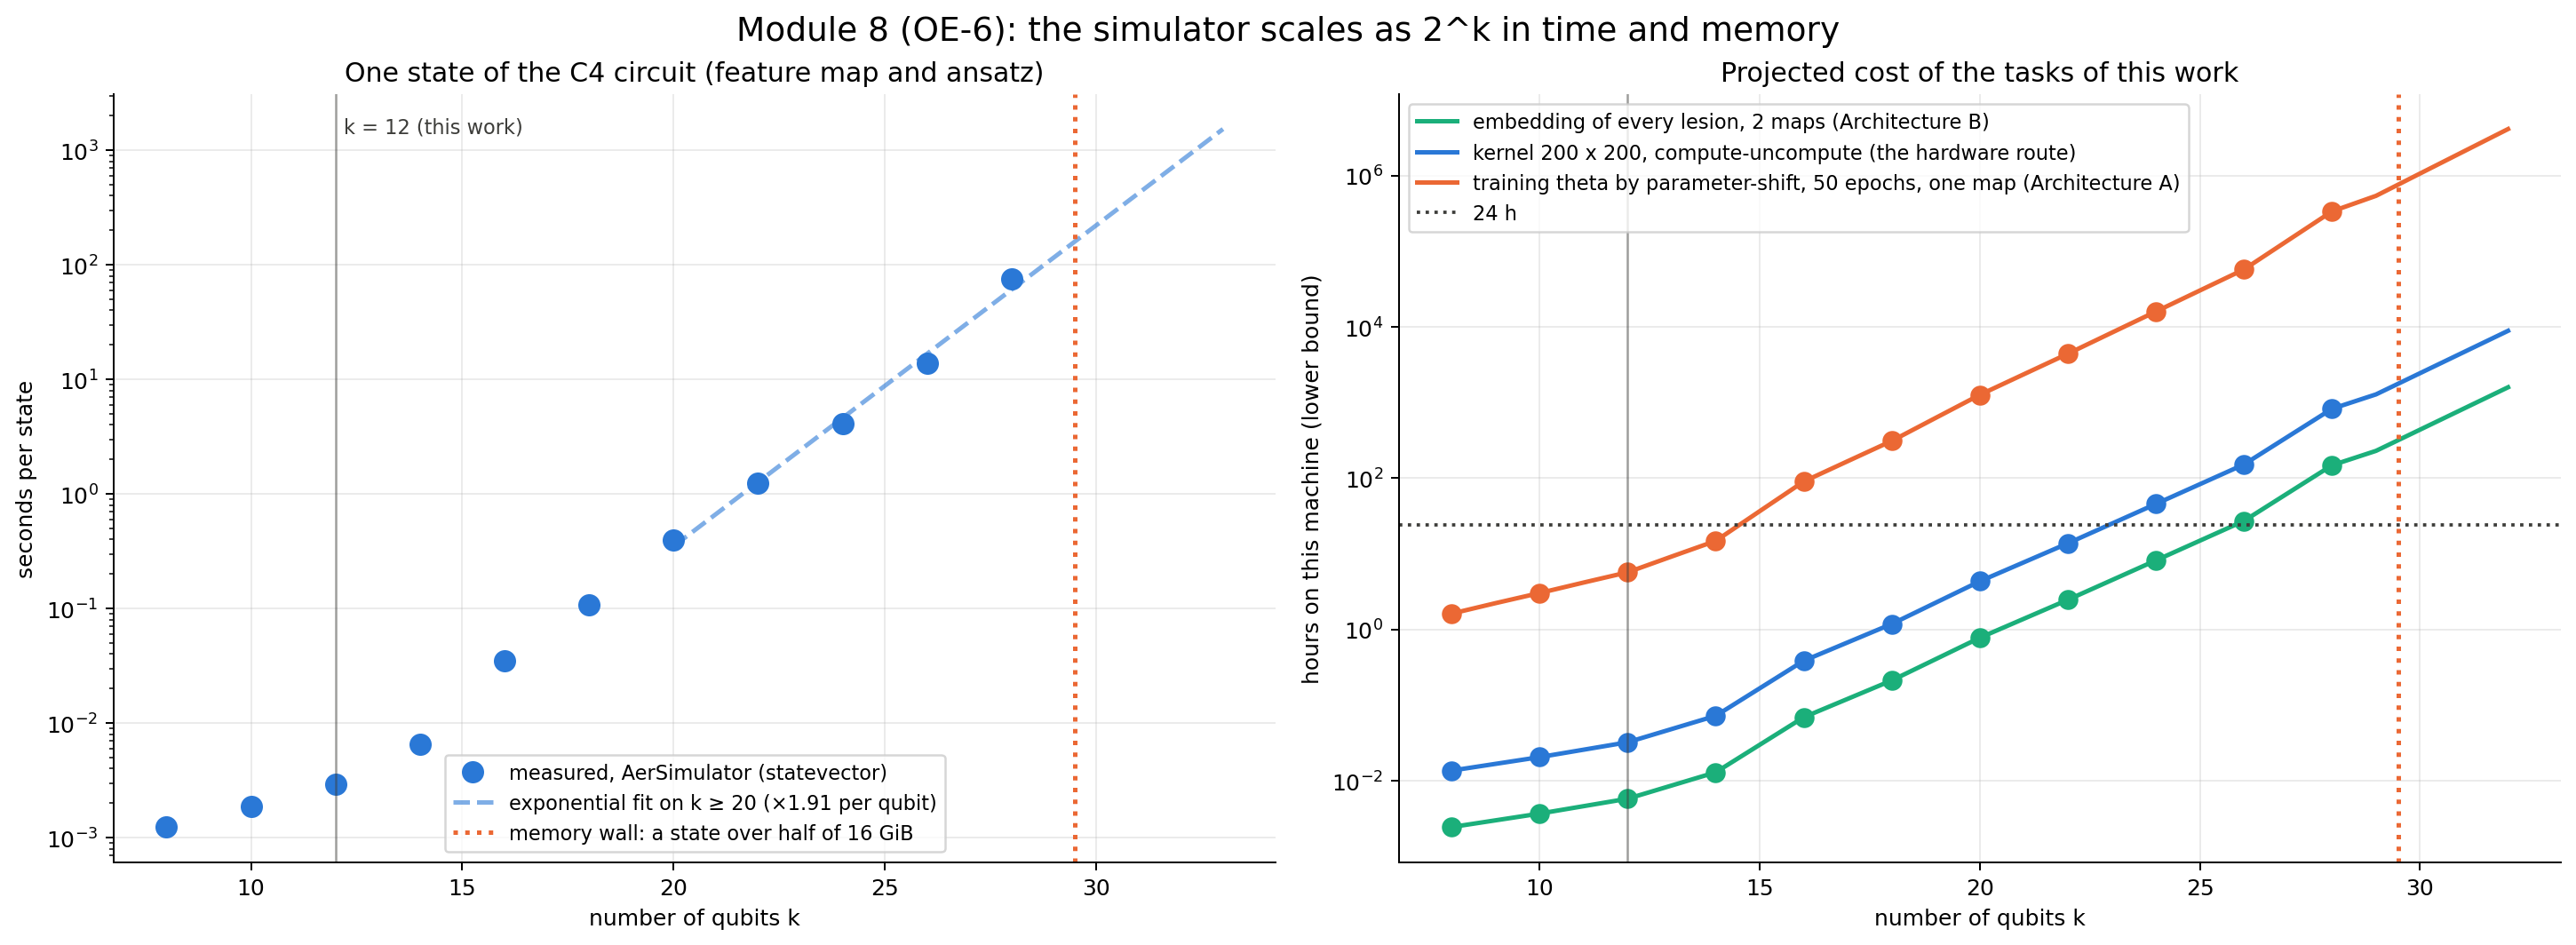
\includegraphics[width=\textwidth]{Figures/M8_oe6_qubits.png}
\caption{Escalabilidad computacional del simulador de vectores de estado en función del número de qubits ($k$) y proyección de límites temporales y de memoria para tareas del pipeline.}
\label{fig:m8_oe6_qubits}
\end{figure}

% fuente: H-052, H-019, H-037; 8_oe6_shots_embedding.csv, 8_oe6_shots_kernel.csv, 8_oe6_resumen.csv
El impacto del número finito de disparos (\textit{shots}) sobre las representaciones locales $\langle Z_i \rangle$ y las matrices de kernel se modeló mediante muestreo multinomial ideal sobre las probabilidades teóricas exactas. En el espacio de \textit{embedding}, la medición con 1\,024 disparos induce un ruido estocástico que representa el 55\,\% y el 65\,\% de la dispersión entre lesiones en C4 (masas y calcificaciones, respectivamente), y el 17\,\% en C5. Se requerirían entre 31\,000 y 44\,000 disparos en C4, y entre 2\,900 y 3\,000 en C5, para reducir el ruido al 10\,\% de la dispersión entre lesiones. No obstante, el clasificador de red neuronal tolera el ruido de medición: con 1\,024 disparos el AUC en validación cruzada retiene prácticamente todo el valor exacto (0.548 frente a 0.565 exacto en C4 masas; 0.630 frente a 0.640 en C4 calcificaciones; 0.565 frente a 0.563 en C5 masas; 0.654 frente a 0.667 en C5 calcificaciones), requiriendo descender a 64 disparos para observar deterioros de hasta 0.08 en AUC.

% fuente: H-052, H-037; 8_oe6_shots_kernel.csv, 8_oe6_resumen.csv
En contraste, la medición del kernel cuántico en hardware físico resulta experimentalmente inviable a escala $c = 1$. Dado que cada elemento del kernel corresponde a la probabilidad binomial de medir el estado cero ($\lvert 0 \dots 0 \rangle$), la concentración exponencial de la fidelidad hace que a 1\,024 disparos por par, el 21.5\,\% de los pares en masas y el 15.7\,\% en calcificaciones lean exactamente cero en C4. Para C5, cuya fidelidad se concentra en órdenes de magnitud menores, el 74.5\,\% de las entradas en masas y el 71.6\,\% en calcificaciones arrojarían una lectura idénticamente nula. Incluso con 8\,192 disparos por par, el 2.5\,\% de los pares en C4 masas y el 1.5\,\% en C4 calcificaciones registrarían cero, mientras que en C5 la fracción de lecturas nulas alcanzaría el 57.0\,\% en masas y el 55.9\,\% en calcificaciones. La mediana de disparos requerida por par para acotar el error relativo al 10\,\% asciende a 46\,000 en C4 masas, 35\,000 en C4 calcificaciones, 3.1 millones en C5 masas y 3.2 millones en C5 calcificaciones. La concentración que deja al kernel sin información de clase es la misma propiedad que impide estimarlo con un número realista de disparos.

\begin{figure}[htbp]
\centering
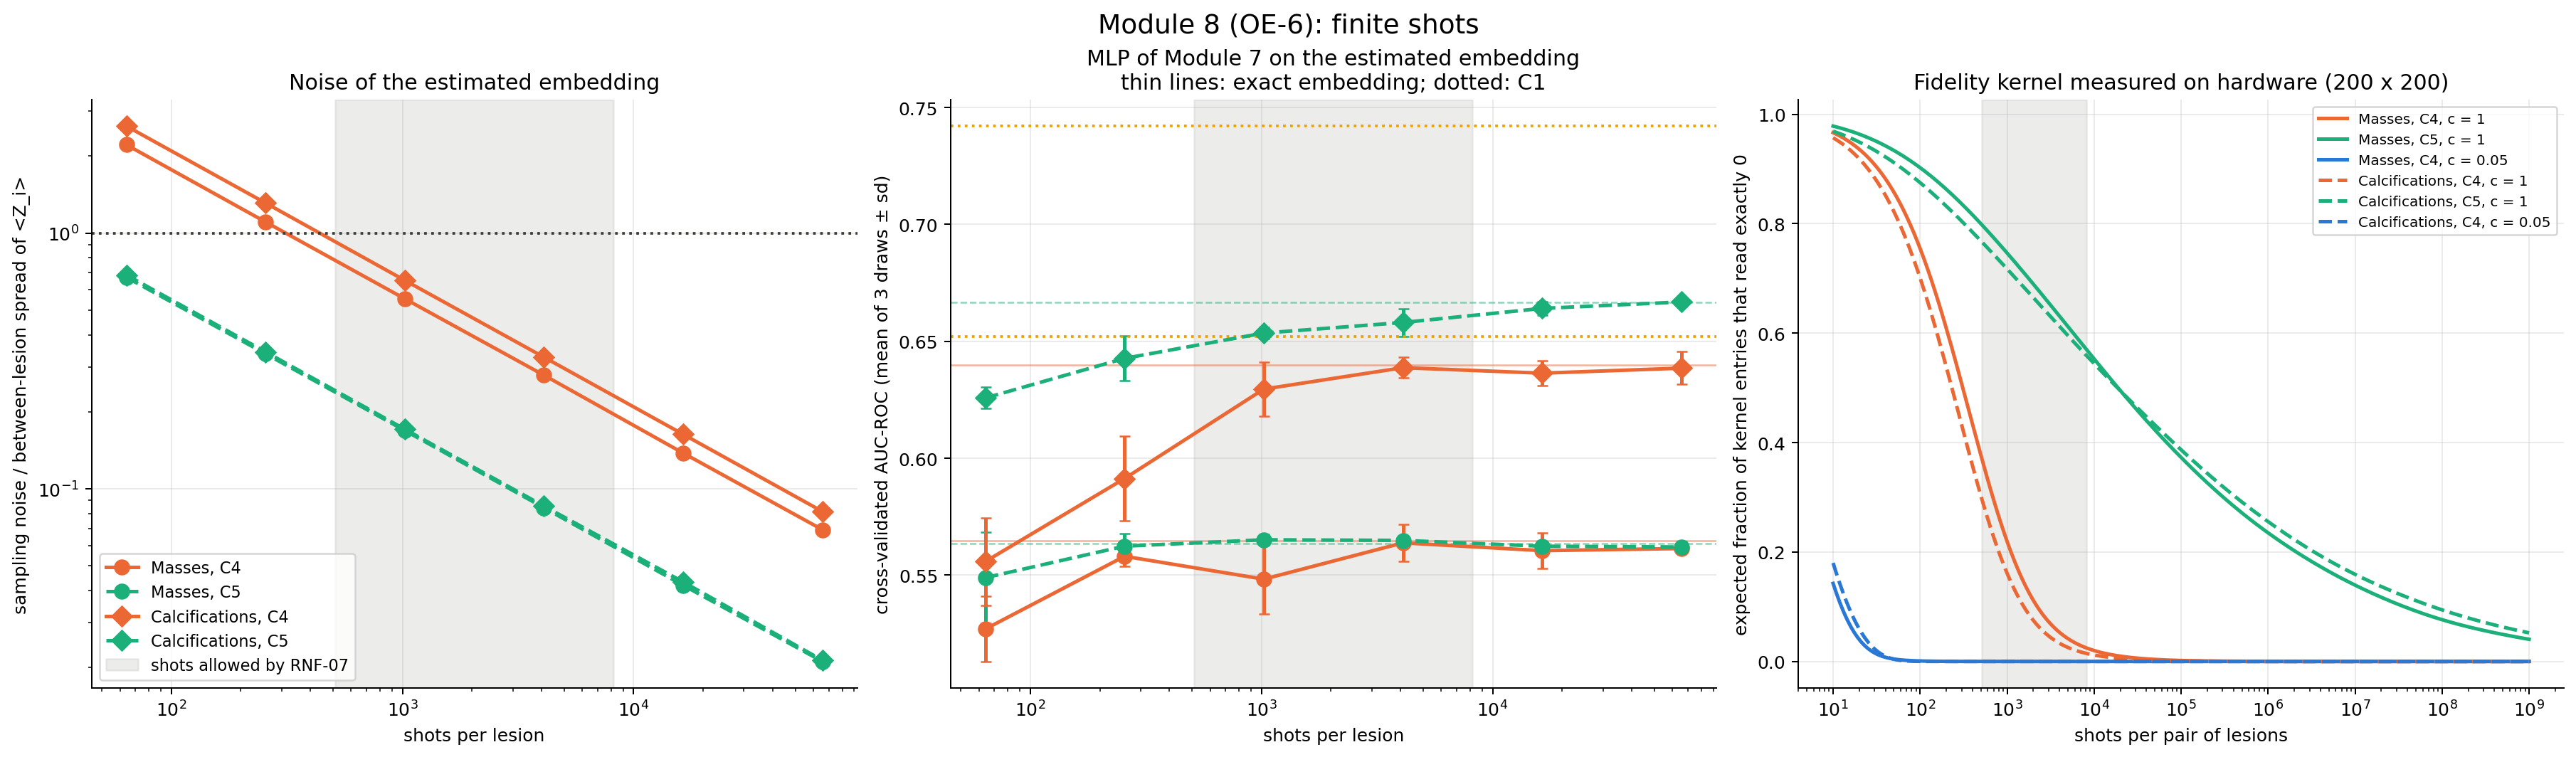
\includegraphics[width=\textwidth]{Figures/M8_oe6_shots.png}
\caption{Efecto del número de disparos (\textit{shots}) sobre la reconstrucción de expectativas en el espacio de estados y sobre la resolución empírica de matrices de kernel cuántico.}
\label{fig:m8_oe6_shots}
\end{figure}
